\documentclass{article}

% Recommended, but optional, packages for figures and better typesetting:
\usepackage{microtype}
\usepackage{graphicx}
\usepackage{subfigure}
\usepackage{booktabs} % for professional tables

% hyperref makes hyperlinks in the resulting PDF.
% If your build breaks (sometimes temporarily if a hyperlink spans a page)
% please comment out the following usepackage line and replace
% \usepackage{icml2018} with \usepackage[nohyperref]{icml2018} above.
\usepackage{hyperref}

% Attempt to make hyperref and algorithmic work together better:
\newcommand{\theHalgorithm}{\arabic{algorithm}}

% Use the following line for the initial blind version submitted for review:
% \usepackage{icml2018}

% If accepted, instead use the following line for the camera-ready submission:
\usepackage[accepted]{mysty}

% The \icmltitle you define below is probably too long as a header.
% Therefore, a short form for the running title is supplied here:
\icmltitlerunning{Newton Methods Coding Project}

\begin{document}

\twocolumn[
\icmltitle{Optimization Method Coding Project 1: \\ Newton Methods}

% It is OKAY to include author information, even for blind
% submissions: the style file will automatically remove it for you
% unless you've provided the [accepted] option to the icml2018
% package.

% List of affiliations: The first argument should be a (short)
% identifier you will use later to specify author affiliations
% Academic affiliations should list Department, University, City, Region, Country
% Industry affiliations should list Company, City, Region, Country

% You can specify symbols, otherwise they are numbered in order.
% Ideally, you should not use this facility. Affiliations will be numbered
% in order of appearance and this is the preferred way.
% \icmlsetsymbol{equal}{*}

\begin{icmlauthorlist}
\icmlauthor{Li, Ziyao}{to}
\end{icmlauthorlist}

\icmlaffiliation{to}{SID: 1500017776, Yuanpei College, Peking University}
%\icmlaffiliation{go}{}
%\icmlaffiliation{ed}{}

%\icmlcorrespondingauthor{Cieua Vvvvv}{c.vvvvv@googol.com}
%\icmlcorrespondingauthor{Eee Pppp}{ep@eden.co.uk}

% You may provide any keywords that you
% find helpful for describing your paper; these are used to populate
% the "keywords" metadata in the PDF but will not be shown in the document
\icmlkeywords{Machine Learning, ICML}

\vskip 0.3in
]

% this must go after the closing bracket ] following \twocolumn[ ...

% This command actually creates the footnote in the first column
% listing the affiliations and the copyright notice.
% The command takes one argument, which is text to display at the start of the footnote.
% The \icmlEqualContribution command is standard text for equal contribution.
% Remove it (just {}) if you do not need this facility.

%\printAffiliationsAndNotice{}  % leave blank if no need to mention equal contribution
\printAffiliationsAndNotice{\icmlEqualContribution} % otherwise use the standard text.

\begin{abstract}
This work focuses on the realization of Newton and Quasi-Newton algorithms. Two test functions are evaluated in this work, namely Box Three-Dimensional Function and Penalty II Function. A Minimal Surface Problem is also solved using Quasi-Newton method. Numerical Experiments are conducted on three formerly mentioned problems. Generally Newton methods takes less iterations than Quasi-Newton methods. SR1 performs poorly on all three problems, making it the least appealing method among all tested algorithms.
\end{abstract}

\section{Line Search}
Two types of line search methods, exact line search (ELS) and inexact line search (ILS) are realized. Here, the exact line search method is mainly discussed. The 0.618 exact search method is realized for conducting ELS. During the process of realizing the algorithm, several problems emerged.

One is that the prior knowledge of $\alpha_0$ is really hard to select. No matter how small the $\alpha_0$ is selected to be, when the gradient $g_k$ of the current point $x_k$ is extremely large or the determinant of the Hesse matrix $G_k$ have relatively small eigenvalues, the function value at $x_{k+1}=x_k+\alpha_0d_k$ can be very large and may overflow. To solve this problem, a detector is added to solve overflow problem. When an overflow is detected, we simply cut the original $\alpha_0$ into $\alpha_0/t$ with given constant $t$, and then solve the problem.

The second problem is the multi-modal problem on $\alpha$. When the searched $\alpha$ leads to $f(x_k+\alpha d)>f_k$, then the step length is not correctly found, and the function must be multi-modal. In this situation, adopting the same strategy, that is, cut the original $\alpha_0$ into $\alpha_0/t$, we can search for a valley region closer to 0, making it more likely to be the valley which $\alpha=0$ is in. Note that such a valley always exists if $d_k$ is the decreasing direction. Continuously doing so until $\alpha<\epsilon$ indicates that $d_k$ is not a decreasing direction, and the algorithm fails. Figure~\ref{fig1} shows a real situation when the second advancement works.

\begin{figure}[ht]
\label{fig1}
\vskip 0.2in
\begin{center}
\centerline{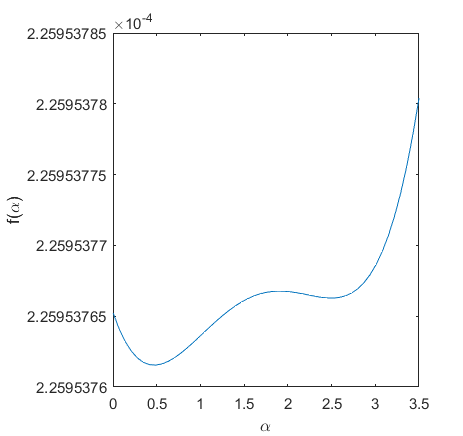
\includegraphics[width=\columnwidth]{graph}}
\caption{Graph of $\tilde{f}(\alpha)=f(x+\alpha d)$ when a multi-modal situation occurs in minimizing Penalty II Function.}
\end{center}
\vskip -0.2in
\end{figure}

\section{Numerical Performance}

Performance of five different methods are tested. Relevant results are shown in Table~\ref{tab1}, ~\ref{tab2}, ~\ref{tab3} and ~\ref{tab4}. Note that the number in the bracket indicates the relative stop criterion. For example, $8(4)$ indicates the algorithm converges after 8 iterations (times of function evaluations) under the criterion
\begin{eqnarray*}
% \nonumber % Remove numbering (before each equation)
  |f_{k} - f_{k-1}| & \le & \epsilon \\
  ||g_{k}||_{\infty} & \le & \epsilon \\
  \epsilon & = & 10^{-4}
\end{eqnarray*}
with default $\epsilon=10^{-8}$.

\begin{table}[t]
\caption{Numerical performance (iterations) of Box 3D Function Minimization Problem.}
\label{tab1}
\vskip 0.15in
\begin{center}
\begin{small}
\begin{sc}
\begin{tabular}{lrrrrr}
\toprule
m & 3 & 5 & 10 & 15 & 20 \\
\midrule
Damp    & 8 & 7 & 7 & 9 & 8 \\
LM & 97 & 8(4) & 1439 & 953 & 760 \\
SR1-B   & 19 & 3(1) & 3(0) & 3(0) & 11 \\
SR1-H   & 19 & 3(1) & 3(0) & 3(0) & 11 \\
DFG-B   & 19 & 9 & 13 & 14 & 11 \\
DFG-H   & 19 & 9 & 13 & 14 & 11 \\
BFGS-B  & 19 & 9 & 13 & 14 & 11 \\
BFGS-H  & 19 & 9 & 13 & 14 & 11 \\
\bottomrule
\end{tabular}
\end{sc}
\end{small}
\end{center}
\vskip -0.1in
\end{table}

\begin{table}[t]
\caption{Numerical performance (feva) of Box 3D Function Minimization Problem.}
\label{tab2}
\vskip 0.15in
\begin{center}
\begin{small}
\begin{sc}
\begin{tabular}{lrrrrr}
\toprule
m & 3 & 5 & 10 & 15 & 20 \\
\midrule
Damp    & 411 & 359 & 357 & 455 & 408 \\
LM & 5429 & 408(4) & 69827 & 48613 & 39526 \\
SR1-B   & 924 & 151(1) & 163(0) & 185(0) & 545 \\
SR1-H   & 924 & 151(1) & 163(0) & 185(0) & 545 \\
DFG-B   & 1022 & 480 & 672 & 801 & 580 \\
DFG-H   & 1022 & 480 & 672 & 801 & 580 \\
BFGS-B  & 944 & 451 & 632 & 705 & 556 \\
BFGS-H  & 944 & 451 & 632 & 705 & 556 \\
\bottomrule
\end{tabular}
\end{sc}
\end{small}
\end{center}
\vskip -0.1in
\end{table}

\begin{table}[t]
\caption{Numerical performance (iterations) of Penalty II Function Minimization Problem.}
\label{tab3}
\vskip 0.15in
\begin{center}
\begin{small}
\begin{sc}
\begin{tabular}{lrrrrr}
\toprule
n & 2 & 4 & 6 & 8 & 10 \\
\midrule
Damp    & - & 4(4) & 3(5) & 103 & 4(3) \\
LM & 5 & 221 & 186 & 104 & 74 \\
SR1-B   & 1(0) & 1(-1) & 7(5) & 2(1) & 2(0) \\
SR1-H   & 1(0) & 1(-1) & 7(5) & 2(1) & 2(0) \\
DFG-B   & 8 & 350 & 1112 & 408 & 763 \\
DFG-H   & 8 & 544 & 1413 & 647 & 637 \\
BFGS-B  & 8 & 373 & 1123 & 862 & 745 \\
BFGS-H  & 8 & 391 & 1355 & 617 & 785 \\
\bottomrule
\end{tabular}
\end{sc}
\end{small}
\end{center}
\vskip -0.1in
\end{table}

\begin{table}[t]
\caption{Numerical performance (feva) of Penalty II Function Minimization Problem.}
\label{tab4}
\vskip 0.15in
\begin{center}
\begin{small}
\begin{sc}
\begin{tabular}{lrrrrr}
\toprule
n & 2 & 4 & 6 & 8 & 10 \\
\midrule
Damp    & - & 212(4) & 161(5) & 5056 & 240(3) \\
LM & 253 & 9838 & 8676 & 5113 & 3827 \\
SR1-B   & 49(0) & 49(-1) & 339(5) & 97(1) & 97(0) \\
SR1-H   & 49(0) & 49(-1) & 339(5) & 97(1) & 97(0) \\
DFG-B   & 377 & 25601 & 80624 & 29354 & 53704 \\
DFG-H   & 377 & 39163 & 101924 & 46186 & 44685 \\
BFGS-B  & 385 & 17723 & 53124 & 40780 & 35421 \\
BFGS-H  & 385 & 18596 & 64215 & 29362 & 37254 \\
\bottomrule
\end{tabular}
\end{sc}
\end{small}
\end{center}
\vskip -0.1in
\end{table}

In the Box 3D problem, although in the first iteration the Hesse matrix is not positive definite and no measures are taken, Damped Newton method gives the best performance. When alternating the Hesse matrix into a positive definite one using LM algorithm, the performance suffers. SR1 method also performs very poorly in this problem. The algorithm fails after several iterations meeting a problem that the direction calculated with the method cease to be a decreasing direction. DFG and BFGS methods give similar performances. By the way, it makes no difference in numerical performance whether a $B_k$ matrix or a $H_k$ one is adopted in the method in this problem.

In the Penalty II problem, Damped Newton method cannot perform after a few iterations due to non-decreasing directions, while a simple LM adjustment gives the best performance among all tested methods. SR1 meets the same problem emerges in Box 3D. Performance of DFG and BFGS are poor in terms of converging speed, while a slightly lowered criterion leads to great improvements. Whether an $H_k$ method or a $B_k$ one is starting to make some differences, however, the differences are slight and the performances are far from stable in two methods to compare which one is better.

\section{Minimal Surface Problem}

Minimal Surface Problem is the Problem 4.3 in \textit{P153}. The problem calculates the minimal surface of a function $v$ on a convex set $D \in R^2$ (or higher dimension) under boundary constraints. In this problem, a differential form of the problem is considered, and the convex set $D$ is limited to a square (rectangular) region for the convenience of grid-differentiation.

Figure~\ref{fig2} and ~\ref{fig3} shows an instance of the process. Figure~\ref{fig2} shows the initial value of $v$ and Figure~\ref{fig3} shows the final output. It proves the algorithm to function since the plane in Figure{fig3} is obvious the minimal solution.

\begin{figure}[ht]
\label{fig2}
\vskip 0.2in
\begin{center}
\centerline{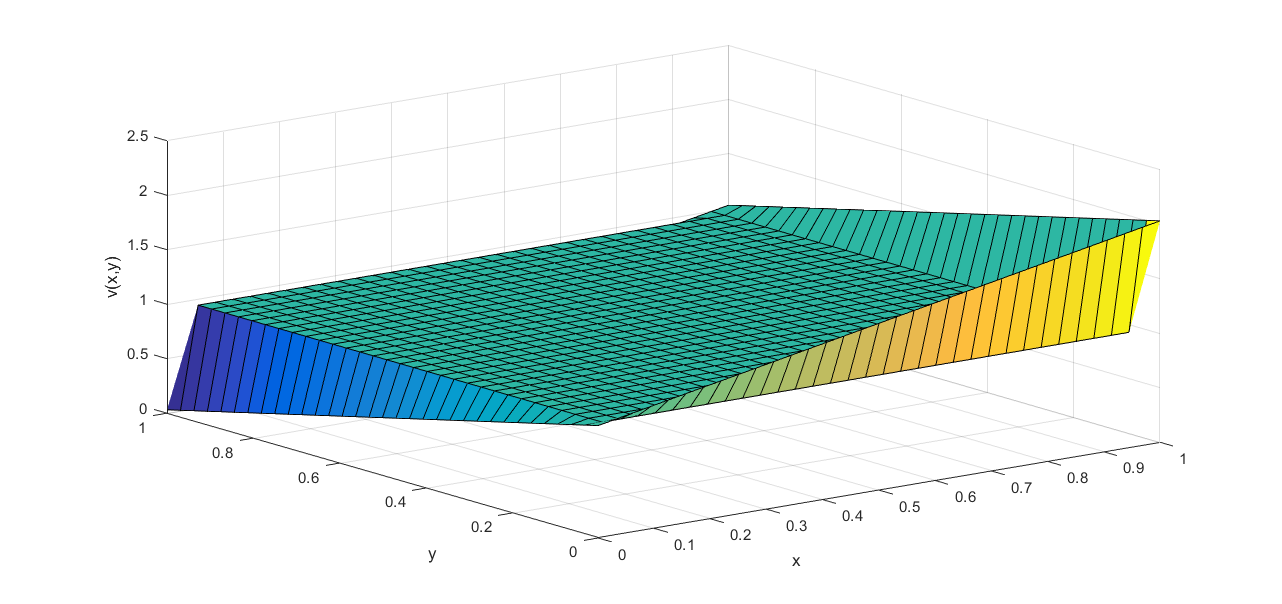
\includegraphics[width=\columnwidth]{init}}
\caption{Graph of linear boundary constraints and initial points with $v(x,y)=1$.}
\end{center}
\vskip -0.2in
\end{figure}

\begin{figure}[ht]
\label{fig3}
\vskip 0.2in
\begin{center}
\centerline{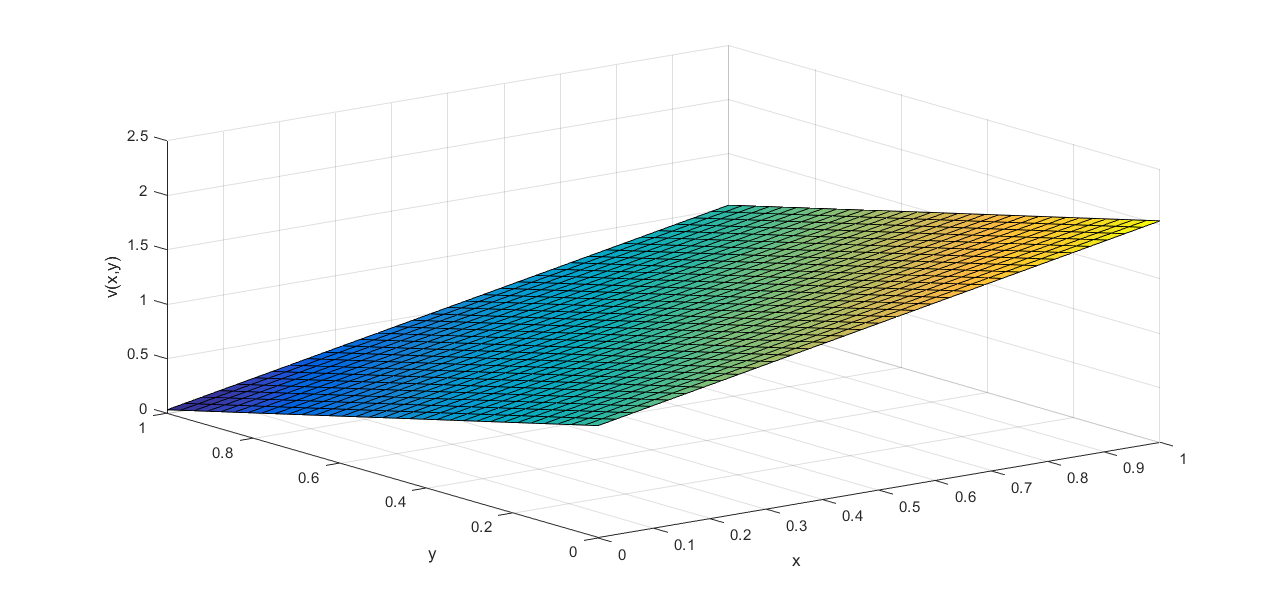
\includegraphics[width=\columnwidth]{rst}}
\caption{Graph of linear boundary constraints and calculated minimal surface.}
\end{center}
\vskip -0.2in
\end{figure}

A comparison of numerical performance of 5 pre-defined types are compared using different algorithms. Detailed definition of the boundary constraints can be found in the relevant codes with coded types. The grid is defined to be $32 \times 32$, i.e. the problem is a 961-dimensional optimization problem. The stop criterion is set to be $10^{-6}$. All seven result graphs are saved in "plots \& results" folder.

The results shows that Newton methods uses a lot less iterations to reach convergence. However, since a differential method is used to approximate the Hesse matrix at a given point, the times of evaluating $f$ is at the same level as Quasi-Newton methods. SR1 still doesn't perform well on this problem, failing to figure out decreasing directions after approximately 300 iterations, when the situation is far from achieving stop criterion.
DFG and BFGS also performs similarly.

\begin{table}[t]
\caption{Numerical performance (function evaluation times) of Penalty II Function Minimization Problem.}
\label{tab4}
\vskip 0.15in
\begin{center}
\begin{small}
\begin{sc}
\begin{tabular}{lrrrrrrr}
\toprule
Type & 0 & 1 & 2 & 3 & 4 \\
\midrule
Damp(iter)    & 5 & 5 & 6 & 5 & 5 \\
DFG(iter) & 102 & 85 & 89 & 97 & 69 \\
BFGS(iter)   & 101 & 84 & 88 & 96 & 70 \\
Damp(feva)   & 5971 & 5985 & 6985 & 5983 & 5985 \\
DFG(feva)   & 5694 & 4554 & 4759 & 5250 & 3504 \\
BFGS(feva)  & 4741 & 4078 & 4289 & 4681 & 3423 \\
\bottomrule
\end{tabular}
\end{sc}
\end{small}
\end{center}
\vskip -0.1in
\end{table}

\end{document}


% This document was modified from the file originally made available by
% Pat Langley and Andrea Danyluk for ICML-2K. This version was created
% by Iain Murray in 2018. It was modified from a version from Dan Roy in
% 2017, which was based on a version from Lise Getoor and Tobias
% Scheffer, which was slightly modified from the 2010 version by
% Thorsten Joachims & Johannes Fuernkranz, slightly modified from the
% 2009 version by Kiri Wagstaff and Sam Roweis's 2008 version, which is
% slightly modified from Prasad Tadepalli's 2007 version which is a
% lightly changed version of the previous year's version by Andrew
% Moore, which was in turn edited from those of Kristian Kersting and
% Codrina Lauth. Alex Smola contributed to the algorithmic style files.
